\chapter{INTRODUCTION (WIP)}

\sepfootnotecontent{fn:path-of-exile}{Path of Exile (Grinding Gear Games, 2013). Computer Game. Microsoft Windows.}

\sepfootnotecontent{fn:diablo}{Diablo (Blizzard Entertainment, 1996). Computer Game. Microsoft Windows.}

\sepfootnotecontent{fn:dark-souls}{Dark Souls (FromSoftware, 2011). Video Game. PlayStation 3, Xbox 360, Microsoft Windows, PlayStation 4, Xbox One, Nintendo Switch, PlayStation 5.}

\sepfootnotecontent{fn:hack-and-slash}{Footnote: What are Hack and Slash Games}

\sepfootnotecontent{fn:checkpoints}{Footnote: What are Checkpoints}

\sepfootnotecontent{fn:boss-fights}{Footnote: What are boss fights}

\sepfootnotecontent{fn:mario-kart}{Footnote: What is Mario Kart}

\sepfootnotecontent{fn:half-life}{Footnote: What is Half-Life}

\sepfootnotecontent{fn:resident-evil-4}{Footnote: What is Resident Evil 4}

\sepfootnotecontent{fn:god-hand}{Footnote: What is God Hand}

\sepfootnotecontent{fn:speedrunners}{Footnote: What are speedrunners}

% ==========================================================
% About the PROBLEM
% ==========================================================

% Game Designers have to decide between large audience or niche
% For broad audience, lean towards casual players with well known features & trends
% For niche games, explore new features & create complex systems
Game Designers are often riddled by the trade off of either appealing to the largest audience possible or entertaining the preferences of a niche. When creating games for a broad audience, game designers lean towards the preferences of casual players, using predefined and well-known features to take advantage of popular trends in a game genre. When creating niche games, designers often express more freedom, exploring new features, mixing older ones and creating complex systems that are well received by the target audience. This can be seen in \emph{Path of Exile}\sepfootnote{fn:path-of-exile}, which uses mechanics previously explored by predecessor games such as \emph{Diablo}\sepfootnote{fn:diablo} and innovates by combining new features with what was already proven to be successful.

% Making game for a niche can strengthen it's core characteristics, vision, aesthetics
% One of the best examples for this is Dark Souls
Tailoring a game to a specific niche during the conceptual phase of development is a valid approach to solidifying its core vision, mechanics and aesthetics, as having well defined delimiters to design decisions simplifies the conception of new systems and promotes a focused and iterative improvement process. One of the most notable examples of successful games that were originally targeted for a niche audience is \emph{Dark Souls}\sepfootnote{fn:dark-souls}, a challenging \emph{Hack and Slash}\sepfootnote{fn:hack-and-slash} RPG (Role-Playing Game) which is considered one of the most influential games of all time and  the origin of the \emph{Souls-like} game genre \cite{BOOK_DarkSoulsBeyondTheGrave}.

% Dark Souls has been prominently discussed due to its difficulty
% Completion rate of 26% even with video tutorials and guides on how to play
% Players report Dark Souls to be frustrating and give up
While incredibly successful and influential, Dark Souls has been the protagonist of multiple discussions regarding difficulty and accessibility in games through the last decade due to its challenging nature in terms of game design \cite{ONLINE_GettingWrongDarkSouls}. In Dark Souls, players are severely punished for committing even the smallest mistakes, and if defeated will repeatedly have to play through the same sections of the game due to sparsely positioned \emph{checkpoints}\sepfootnote{fn:checkpoints} (named "bonfires" in the game world). As a result, a percentage as low as 26\% of the consumer base has completed the game after 10 years since its release \cite{ONLINE_ApproachabilityFixDarkSouls}, with multiple online resources such as video tutorials and guides being published to assist new players. Many players report Dark Souls to be a frustrating, unenjoyable experience and decide to give up before being immersed and engaged in the game's world and lore \cite{ONLINE_ToughLoveDarkSoulsDifficulty}.

% Controversy of dark souls created discussions on difficulty vs experience
The controversy around Dark Souls served as a catalyst to push forward discussions regarding the impact of game difficulty in player experience. For a game to successfully bring enjoyment to the player, it has to cause the player to become involved and focused while playing \cite{ARTICLE_FlowInGames}. Therefore, one of the critical factors of game design is the ability of a game to make the players immersed in its experience. 

% Flow is the most popular concept regarding immersion
% Flow is partially determined by the challenge in regards to skill 
The most established concept in academic literature pertaining player immersion and focus is the theory of Flow \cite{BOOK_Flow}. Flow is the state in which a player is completely immersed within the experience of a game. The ease to reach the state of Flow is determined by, among other properties, the challenge of a game in contrast to the skill of its player. According to the Theory of Flow, for a player to become completely immersed in the experience of a game, the difficulty of the game should match the skill level of the player. A game that is not challenging at all will bore the player. A game that is too challenging might cause anxiety and result in the player giving up.

% Game balanced for all would be the best solution
% One of the common approaches in the industry is to have presets of difficulty
A game with balanced challenge for all players would ideally be the best solution. In practice it is difficult to accomplish such, risking an unsatisfactory result for each type of audience where either beginner players will be frustrated by the level of challenge or veteran player might find a game too easy. One of the most common approaches to attempt to balance games to multiple audiences is to implement multiple presets of difficulty curves such as \emph{Easy}, \emph{Normal} and \emph{Hard} game modes that modify specific in-game parameters to provide an easier or more challenging experience that can be chosen by the player.

% Issues with difficulty presets:
%    - If a player has not experienced the game beforehand or even another game of the same genre, they might not be able to tell their skill level before choosing a difficulty. 
However, using difficulty presets has multiple issues related to player assessment and choice of difficulty curves. First, if a player has no experience with the game beforehand or even with another game of the same genre, they might not be able to correctly assess their own skill level in comparison to the challenge levels proposed by the game designers. Therefore, they might incorrectly select a game mode that is too frustrating or boring and have difficulty being immersed by the experience.

% Games provide easy, normal, hard modes
%    - The game difficulty has to be changed in the middle of a play session, which creates pauses and variations in the game experience that might break immersion.
For this reason, some games provide the option of changing the difficulty mode over the course of a play session, which alleviates the issue but creates pauses and variations in the game experience that might affect player immersion and cause negative effects on the experience. Even worse, the player might be tempted to modify the difficulty to overcome challenges that are designed to be above the overall game difficulty, such as \emph{boss fights}\sepfootnote{fn:boss-fights} -- which further breaks the immersion and the purpose of such sections of a game in regards to player experience.

%    - The player might be motivated to continue to play in the same difficulty level due to their perception of their own skill level, which might not go in accordance with the target skill level intended by game designers
Additionally, when a game employs the possibility of altering difficulty in the middle of a play session, the player might be motivated to continue to play in the same difficulty level due to their perception of their own skill level, which might not be in accordance with the target skill level intended by game designers. In that case, the player might be frustrated by the fact that their expectations of the challenge level of a specific mode might not meet the actual difficulty proposed by game designers.

%    - Player skill can be defined through multiple perspectives
%        - A player might be able to take good decisions but not have a good reaction time
%        - Conversely, a player might have a good reaction time but not understand which approach they should take to overcome a challenge.
%        - A player might make a better use of one game mechanic in relation to others, and become addicted to using it repeatedly, which causes the game to become repetitive
Furthermore, there is still the issue of defining player skill to appropriately create difficulty curves, which can be done through multiple perspectives since game systems might involve mechanics that require knowledge of different concepts or decision-making processes. For instance, a player might be able to take good strategical decisions in a combat situation, but be unable to execute such decisions due to a poor reaction time. Conversely, a player might have a good reaction time but not possess a sufficient understanding of the approach that should be taken to overcome a challenge. A player might also make better use of a specific game mechanic in relation to others and feel motivated to use it repeatedly due to their success when using it. This might cause the game to become repetitive, as the game does not appropriately provide the player with situations that incentivize the use of varied mechanics or strategies.

% ==========================================================
% About what was already done in DDA (in research)
% ==========================================================

\section{Adaptive Systems In Research}

To directly deal with the issue of game difficulty without relying on player expectations and choices, it is possible to automatically adapt a game over the course of a play session satisfy the specific needs of each player. Such a model can be achieved through \emph{Adaptive Game Systems} \cite{ARTICLE_PlayerCentredGameDesign}, where the game monitors the actions performed by the player to define a player \emph{profile} and provide customized responses, calculates the efficiency of player decisions to analyze player \emph{performance} and adjust difficulty, and adapts its content based on player \emph{preferences} to provide an experience tailored to the expectations of a player.

% General description of research in adaptivity covered in this work
%   - Probabilistic model
Research conducted on AGS (Adaptive Game Systems) has tackled the issue of adapting game difficulty to players through multiple perspectives by using different methods for monitoring and classification of players, as well as different philosophies for the adjustments that should be performed to modify the difficulty curve. Methods that create a \emph{probabilistic model} such as the work in \cite{article_casefordda} perform proactive adjustments based on the probable outcomes from a specific in-game event faced by the player to avoid game state "loops", where the player would repeatedly play through the same game sections or perform the same set of actions.

%   - Affect-based
Alternatively, \emph{affect-based} methods such as the work in \cite{article_affectivedda} attempt to recognize the affective state of a player by monitoring physiological signals that can infer the anxiety level of players, and then adjust the difficulty level accordingly. This is a reactive approach to stimuli gathered from the player, and can be directly related to the concept of \emph{Flow} where we attempt to avoid states in which a player might become too frustrated or bored with the game experience.

%   - Reinforcement Learning
Finally, \emph{learning-based} methods such as the work in \cite{article_adaptivebehaviorai} attempt to create a novelty approach to adjustments by adapting AI agent behaviors through learning-based algorithms such as \emph{reinforcement learning}, where the game designer has a reduced responsibility in tailoring the values modified by the adjustment system. This type of approach requires the employment of offline learning techniques, where AI agents are rigorously trained by performing extensive play sessions against non-learning AI agents, or by gathering a sufficient amount of gameplay data from human players.

% ==========================================================
% About What was NOT Resolved and is OPEN (In Research)
% ==========================================================

% Research was performed in simple games with limited interactivity and simple mechanics and systems
While previous research on adaptive methods for game difficulty provided a variety of novelty approaches that have yet to be explored by the video game industry, it is important to note that the implemented methods were experimented on simple games with limited interactivity or complexity. Therefore, research on AGS has yet to explore the results of adaptivity in the environment of commercial solutions, where games feature complex functionality and a variety of game mechanics and systems.

% Previous research did not tackle the issue of providing automated accessibility in games that are purposed to be difficult by design
Additionally, previous adaptive methods did not explore the possibility of providing automated accessibility and difficulty parameters in games that are purposed to be difficult by design, such as Dark Souls. By attempting to integrate dynamic difficulty to games in which overcoming difficult challenges is part of the proposed experience, it would be possible to measure the effectiveness of adaptation to increase their viability to beginner players. Simultaneously, it would also be possible to leverage the side effects of adaptive solutions to players which were the original audience targeted by game designers.

% AGT has to be integrated smoothly to the game development process, and must be an active part of the iterative methodology for game design
Lastly, for Adaptive Game Systems to be viable in industry-based game development, they should have the capacity to be integrated without introducing friction into the game development process. Instead, they should be an active part of the iterative method which is used by game design. The monitoring, classification and adjustment algorithms, as well as the parameters used for such adjustments, should be able to be iteratively modified as the design of the game changes or as play testing sessions indicate flaws in the balance of difficulty curves. 

% Learning-based and affect-based methods are not viable
Therefore, \emph{learning-based} methods would be unable to satisfy the nature of the iterative design process, as they require agents to be extensively tested over fixed parameter values to properly reflect the balance of the game. In the same sense, \emph{affect-based} methods would not be viable to implement in the vast majority of games, as the input devices used by gaming platforms are not commonly able to track physiological signals.

% ==========================================================
% About DDA solutions in the game industry
% ==========================================================

\section{Adaptive Systems In Industry}

% Description of techniques used in the industry
%   - Distribution of resources
As for approaches to dynamic difficulty implementation that were popularized in the video game industry, one of the most common employed approached is the \emph{dynamic resource distribution} which is presented in \emph{Mario Kart}\sepfootnote{fn:mario-kart} and \emph{Half-Life}\sepfootnote{fn:half-life}, where the game monitors player performance and distributes items based on the current necessity of the player at a given point. For instance, in Half-Life if a player is low on health and opens an item container such as a box, the game prioritizes the distribution of health recovery items by increasing the chance of such an item spawning.

%   - Dynamic AI RE4
Another popular type of approach in the video game industry is the use of dynamic AI (Artificial Intelligence) agent behaviors, where the player monitors the frequency of player actions to modify the behavior of enemies in response, so that the player is unable to use the same strategy repeatedly over the course of the game. Such an approach can be seen in \emph{Resident Evil 4}\sepfootnote{fn:resident-evil-4}, where if players are accurately able to shoot enemy heads to deal more damage, enemy entities will start to be instantiated with protective helmets or perform defensive maneuvers to avoid shots.

%   - Explicit approach in God Hand
A less popular approach to dynamic difficulty that was briefly experimented in the industry was the use of \emph{explicit adaptivity}, where the existence adaptive system is made apparent to the player through the user interface, and the increase or decrease of game difficulty is a \emph{gamified} system in itself. This can be seen in the game \emph{God Hand}\sepfootnote{fn:god-hand}, where as players successfully defeat enemies while taking a minimal amount of damage, a "difficulty meter" is constantly increased, making enemy animations faster and increasing the amount damage dealt to the player. As a reward, the player receives an increased amount of points for defeating enemies in higher difficulty levels, which can be spent on unlocking multiple game features. 

% ==========================================================
% About the problems with solutions in the game industry
% ==========================================================

% Item distribution and behavioral changes can be interesting, but as players progress through the game they start recognizing patterns, and eventually the system becomes exploitable
The difficulty adjustment methods implemented in commercial games often prove to be effective when attempting to alleviate the difficulty for beginner players. However, as players become more experienced in a game and accustomed to the implemented systems, they start to recognize patterns which might give them advantages while playing. For instance, in Resident Evil 4 it is common for \emph{speedrunners}\sepfootnote{fn:speedrunners} to miss shots on purpose in order to restrict the behavioral patterns of enemies and make the game easier.

As an adaptive system becomes apparent to the player, they will modify their play style to exploit the system in their advantage. This produces negative side effects to player immersion, as the player becomes preoccupied with a specific type of strategy in order to "beat the system", instead of performing the actions that are best suited to a specific situation. Therefore, it is important that adaptive systems are abstracted to the player to provide a more immersive experience, and thus there is an incentive to explore more ambiguous or complex adjustments that can not be easily perceived by players.

% ==========================================================
% Outline of proposition
% ==========================================================

\section{Implementation and Scope}

% This work attempts to use characteristics of AGS research in the environment of a commercial Game
This work attempts to use the knowledge acquired from previous research on AGS in the environment of a commercial game, where we attempt to adapt the metrics and adjustments to the iterative nature of the game design process in video games development. We attempt to apply such techniques to a game that is designed to be challenging as a standard, trying to alleviate the difficulty curve so that beginner players experience less frustration in the process of becoming accustomed to game mechanics and systems.

% Implementation of a replica of Dark Souls consisting of the "core" experience
As an object of study, we implement a computer game that contains a subset of the mechanics, systems and aesthetic elements presented in Dark Souls. Our implementation was designed to replicate the core experience of Dark Souls, where the most relevant mechanics and features were leveraged into a simplified game with reduced scope. We also attempt to replicate the aesthetic elements of Dark Souls by using 3D (three-dimensional) models, visual effects and sound effects that can properly compose a \emph{Dark Fantasy} setting. Figure \ref{fig:implementation-bright-souls} exemplifies a combat situation in our implementation, where the player faces a challenging enemy type based on the enemies presented in the original Dark Souls game.

\begin{figure}[!ht]
    \caption{A screen capture of \emph{Bright Souls}, our implementation of a game based in \emph{Dark Souls} game with a subset of the mechanics and systems presented in the original game.}
    \begin{center}
        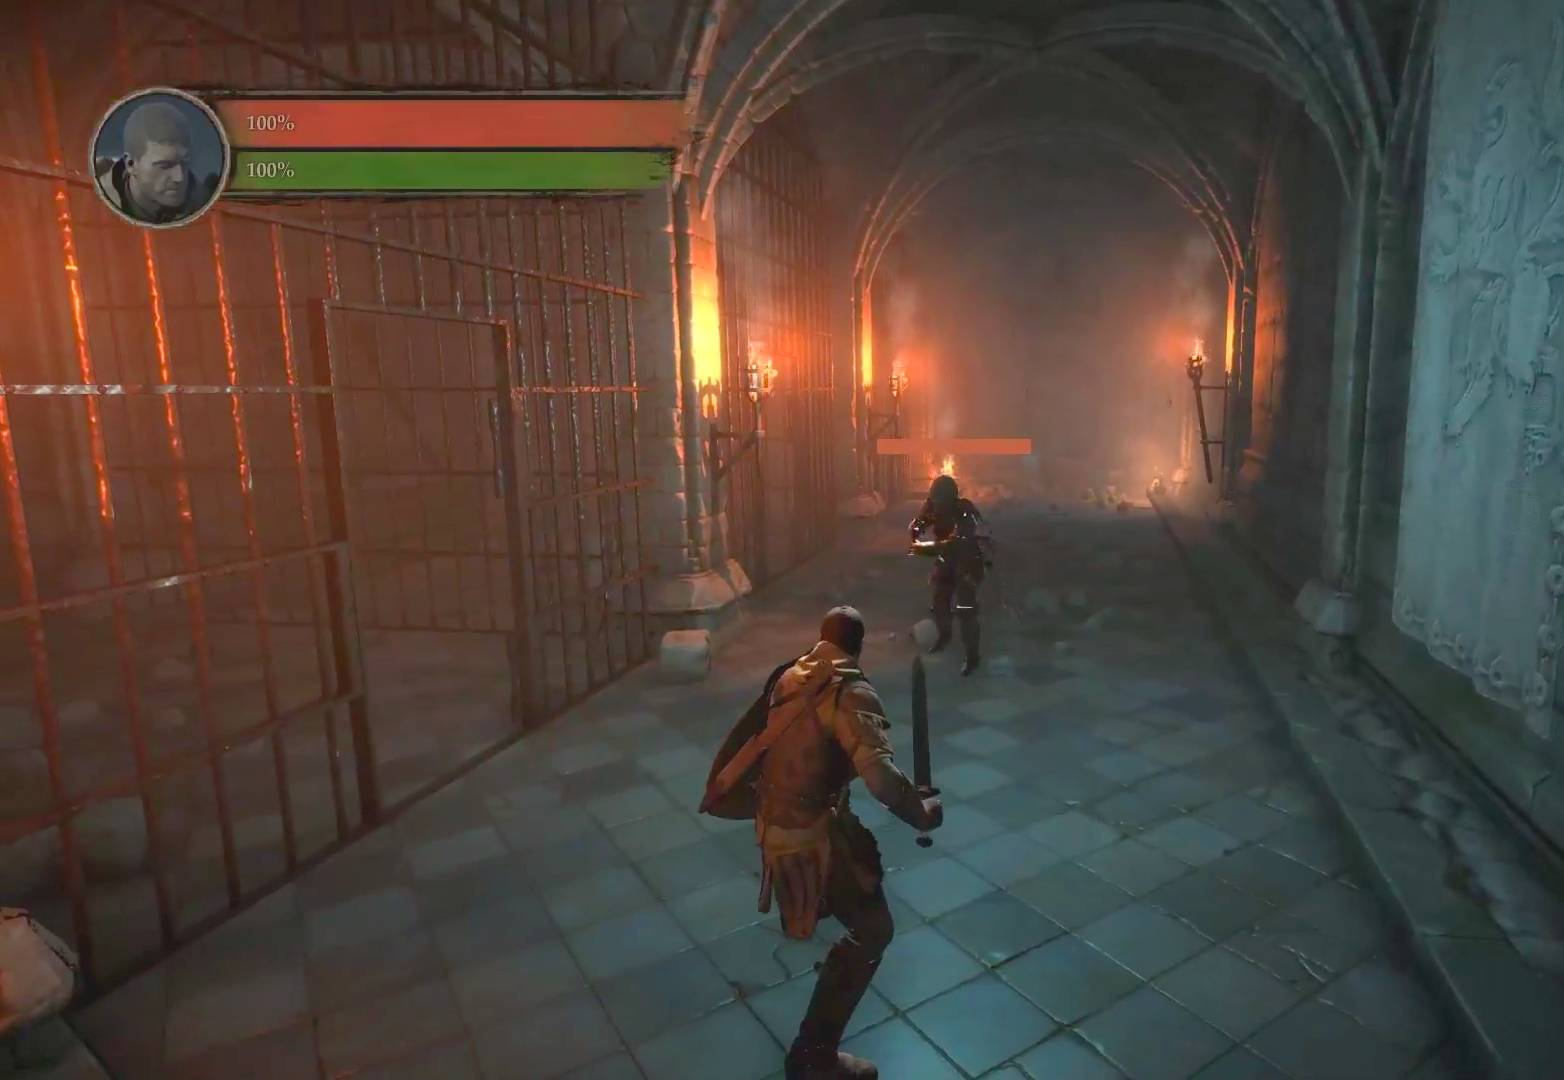
\includegraphics[width=30em]{figures/fig-bright-souls.jpg}
    \end{center}
    \legend{Source: Screen capture performed by the authors of the implementation presented in this work.}
    \label{fig:implementation-bright-souls}
\end{figure}

% Definition of difficulty as an N-dimensional set of parametric difficulty adjustment values
To adapt the difficulty curve of Dark Souls to a broader audience with a variety of skill levels, we attempt to define game difficulty as an N-dimensional set of parametric difficulty adjustment values, which can be dynamically adjusted over the course of a game session to better satisfy the needs of specific player types. In sequence, we define a range of adjustment parameters that can be independently configured so that the player can focus on improving their performance when using specific mechanics and systems rather than the game as a whole.

% Statistical approach to metrics and adjustments to properly integrate into the iterative nature of the game design process
To provide a novelty approach to the implementation of Adaptive Game Systems which can be appropriately integrated into the game development process, we employ a statistical approach to the use of player metrics when performing adjustments, where we define a series of thresholds define conditions to the application of each adjustment value. While this approach is loosely related to the work developed in \cite{article_casefordda}, the threshold-based conditions presented in our implementation simplify the iterative process of game development, where game designers are able to adjust threshold conditions and adjustment values after analyzing the results of single or multiple play sessions without causing negative effects on the adjustment algorithms.

% Adjustments are chosen to be harder to perceive by players and provide an abstracted difficulty curve where players face higher challenges levels as they overcome each encounter
The adjustments in our implementation were elected based on analysis of the difficulty factors in the original Dark Souls game, as well as on the abstraction level in relation to player perception of difficulty. Therefore, we argue that our adjustment parameters are harder to perceive by players in comparison to common approaches employed in commercial games, while also providing interesting modifiers that game designers can work with to customize difficulty curves.

% Comparison to difficulty as a set of preset configurations
To compare the effectiveness of implementing difficulty as an N-dimensional set of adjustable parameters in comparison to predefined difficulty configurations that are used commercial games, we perform an experiment where players of multiple skill levels are monitored while playing through two versions of our game: one with fixed values for difficulty parameters which are set by using a \emph{player classification survey} to select one of multiple pre-configured difficulty presets; and another where the game dynamically adjusts difficulty parameters after each level based on player performance and their most common actions.

% ==========================================================
% Summary of each chapter
% ==========================================================

\section{Structure of This Work}

% Related work

% Analysis of Object of Study

% Implementation and Design

% Experiment Methodology and Results

% Discussion

% Conclusion